% 1977 年广西百色卷（理科）参考题 2（源卷「选作题」第 2 题）：半径 10cm、
% 圆心角 120° 的弓形内接正方形 CDEF，半径 OP⊥FE 交 FE 于 N、AB 于 M（按源卷第 6 页布局）
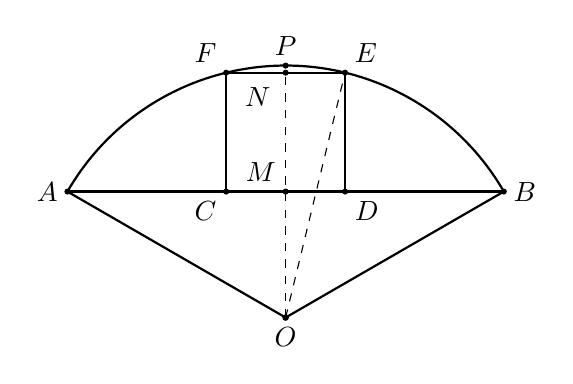
\begin{tikzpicture}[scale=1.0]
  % O 为圆心，R=3.2cm；A、B 为弦端点，C、D 在弦上，F、E 在弧上，P 为弧中点
  \coordinate (O) at (0,0);
  \coordinate (A) at (-2.771,1.6);
  \coordinate (B) at (2.771,1.6);
  \coordinate (M) at (0,1.6);
  \coordinate (C) at (-0.755,1.6);
  \coordinate (D) at (0.755,1.6);
  \coordinate (N) at (0,3.110);
  \coordinate (F) at (-0.755,3.110);
  \coordinate (E) at (0.755,3.110);
  \coordinate (P) at (0,3.2);
  \draw[thick] (O)--(A);
  \draw[thick] (O)--(B);
  \draw[thick] (A)--(B);
  \draw[thick] (A) arc (150:30:3.2);
  \draw[thick] (C)--(F)--(E)--(D);
  \draw[dashed] (O)--(P);
  \draw[dashed] (O)--(E);
  \fill (O) circle (1.2pt) node[below] {$O$};
  \fill (A) circle (1.1pt) node[left] {$A$};
  \fill (B) circle (1.1pt) node[right] {$B$};
  \fill (P) circle (1.1pt) node[above] {$P$};
  \fill (F) circle (1.1pt) node[above left] {$F$};
  \fill (E) circle (1.1pt) node[above right] {$E$};
  \fill (C) circle (1.1pt) node[below left] {$C$};
  \fill (D) circle (1.1pt) node[below right] {$D$};
  \fill (M) circle (1.1pt) node[above left] {$M$};
  \fill (N) circle (1.1pt) node[below left=2pt] {$N$};
\end{tikzpicture}
